\section{The Benchmark Data Set} \label{sec:data-set}
This section focuses on presenting the data set that was the basis for the methods developed in this chapter.
The data set was provided by the Istituto Cantonale di Patologia and preprocessed in order to be used to learn a Bayesian Network.

\subsection{The Medical Partner: Istituto Cantonale di Patologia} \label{subsec:istituto-cantonale}
Istituto Cantonale di Patologia (ICP)\footnote{\url{https://www4.ti.ch/dss/dsp/icp/istituto/}} is an institute based in Locarno that is specialised in the histological analysis of tissue samples received from private patients, clinics and hospitals, mainly in support of cancer diagnosis.
Its Laboratory of Molecular Pathology supports the diagnostic approach to neoplastic diseases through the application of biomolecular and cytogenetics techniques, which focus on understanding the impact of molecular alterations in carcinogenesis.
One of the methods used is Fluorescence in Situ Hybridization (FISH) (see Figure \ref{fig:fish-picture} for an example of the results of this technique) that is able to localise the presence or absence of specific DNA sequences in chromosomes.
These tests are aimed at identifying the precise profile of the cancer cells and thus inform the clinician on the best treatment for the specific patient.

\begin{figure}[htbp]
\centerline{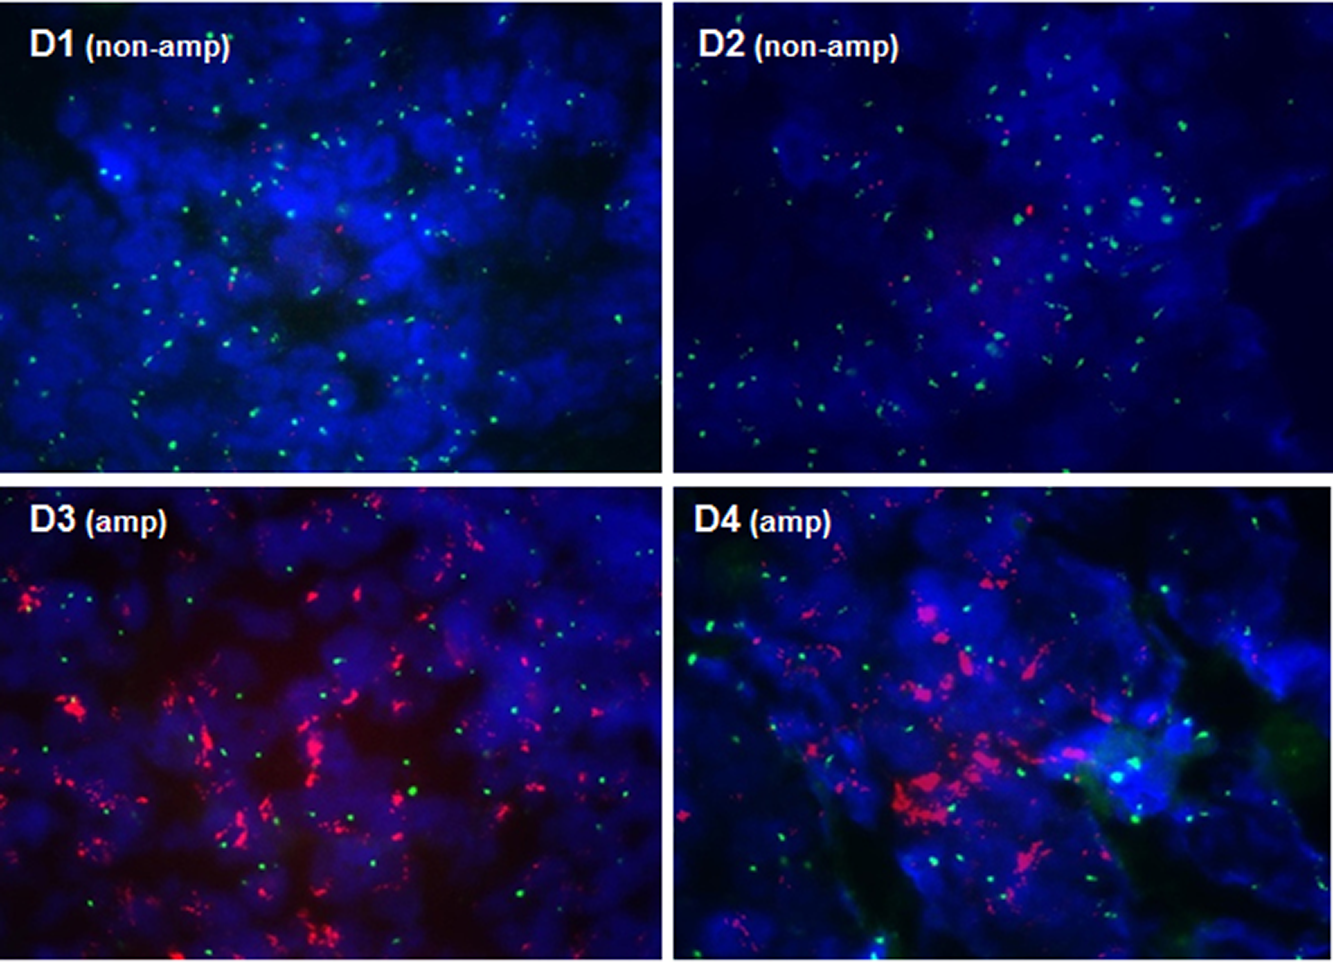
\includegraphics[width=0.8\textwidth]{methodology/images/fish-picture}}
\caption{FISH analysis of HER2 gene expression in samples of breast tumour. The probe mix consists of a mixture of Texas Red-labelled DNA probe against HER2 gene (which is located on chromosome 17) and a fluorescein (green)-labelled probe targeted at the centromeric region of chromosome 17. The upper panels (D1 and D2) show normal expression - 2 green and 2 red signals per cell. The lower panels (D3 and D4) show HER2 amplification whereby there is a clear increase in the red signal. [source: https://www.bioivt.com/fluorescent-in-situ-hybridization-fish/]}
\label{fig:fish-picture}
\end{figure}

Molecular diagnosis is the most recent approach in pathology. It mainly aims to support pathologists in the diagnosis of neoplastic diseases through the employment of molecular biology and cytogenetics techniques and it enables the deep understanding and monitoring of patients' profiles, as well as as defining the prognosis and ad-hoc therapies. All together, it allows the development of an increasingly personalised medicine, also in terms of research (e.g. understanding of pathological mechanisms and thus the possibilities of intervention).
However, it is still limited in its capabilities by the presence of a dishomogeneous information pool, especially in terms of knowledge extraction; a non-uniform data set entails, for the pathologist, an increased cognitive complexity because of having to manage a high number of variables and heterogeneous meaning behind the data; these consequently force to resort to problem decomposition and reduction.

In addition to its clinical support activities, the ICP also carries out scientific research aimed at better understanding certain types of cancers at translational level i.e., at the level of protein synthesis.
In the last ten years, the ICP has published more than 200 peer-reviewed papers and more than 100 works in non-peer reviewed journals and is active at a national and international level.

\subsection{Motivation} \label{subsec:motivation}
The Istituto Cantonale di Patologia already had a collaboration in place with the Dalle Molle Institute for Artificial Intelligence (IDSIA)\footnote{\url{http://www.idsia.ch}} to investigate a series of specific issues, whose details are outside of the scope of this thesis.
The prospect of the work to be carried out in this thesis was deemed of interest because it extended beyond the existing collaboration.
The institute had originally expressed interest in bringing machine learning into their workflow in order to both augment its profiling capabilities for patients and to be able to extract new knowledge from their existing data; this was paired with an attention for more experimental research directions, as the facilitation of human-machine interaction.

Given that the theoretical work carried out in this thesis is, at its core, an investigation into the explainability of Bayesian Networks, collaboration with the Institute provided the precious opportunity to implement a proof of concept system (described in Chapter \ref{chap:methodology} and \ref{chap:results}) based on a real medical data set and, most importantly, opened an opportunity for an \textit{application-grounded evaluation} of it (see Section \ref{sec:evaluation-of-explainability}).

The first contact with the ICP was in January 2019, during a meeting with Vittoria Martin (PhD), molecular cytogenetist, and Luca Mazzucchelli (Dr. Med.), director of the institute.
Since then, the clinicians and researchers of the ICP have been able to validate, from an Explainable AI and clinical relevance point of view, the model software that has been developed.
That is to say, they have validated, to an extent that will be made clear in Chapter \ref{chap:results}, the developed software both in its adherence to established medical literature and in its capacity to support clinical decision making and to surface clarifying explanations of the data set.
This is a great opportunity because the lack of real-world validation of ML systems with real domain experts is one of the prime gaps in the existing xAI literature (as discussed in depth in Chapter \ref{chap:literature-review}).

An example application for a clinician of the ICP, would be ability to \enquote{fill in the blanks} of a patient's profile, as it is not uncommon, for a variety of reasons, to have missing data.
This may be because of degraded or insufficient tissue samples or because some test may not yet be part of the standard diagnostic procedure, even though their importance may already be suggested by clinical research.
In other cases, patients may be missing a result because the specific test had not yet been invented, for example FISH was not available prior to 2010, so an a posteriori inference could be made possible.
Another crucial use may be in understanding and quantifying in an efficacious manner the relationship between clinical variables.
It is not uncommon for some variables to have been observed but for their clinical relevance not to have yet been determined; learning their relationship with other variables could potentially not only help in defining their importance in tracing new patient profiles in terms of diagnostic, prognosis and support in decision making but also in placing them in terms of pathological mechanisms.
These are all examples highlighting the importance of the \textit{inference} capabilities of machine learning and \textit{uncertain reasoning} techniques, but the current work aims to principally address the interfacing of the human user with the software while carrying out these queries.
It is also hoped that facilitating the process of knowledge-extraction may lead towards the confirmation of current scientific theories or may be the first step towards the formulation of novel ones.

\subsection{Provided Data Set}
The provided data set was created by \textit{Registro Tumori Ticino}\footnote{\url{https://www4.ti.ch/dss/dsp/icp/registro-cantonale-dei-tumori/home/}} (Locarno, Ticino) in order to highlight possible new relations between clinical, histopathological and molecular features, as well as to potentially discover novel biomarkers involved in the progression of the disease.
It consists of the histopathological records, over 38 variables of interest, of 3218 breast cancer patients who have been diagnosed between the years 2005 and 2014 within the Ticino canton of Switzerland.
The data set had already been pre-processed by collaborators of IDSIA under supervision of the ICP, with 13 of the variables being dropped because not relevant.
In particular, all variables relating to patients post-treatment were discarded as well as those recording the diagnosis date.
The data set was also anonymised, for obvious privacy issues.
Some of the variables were initially numerical (for example \enquote{FISH}) but all were converted to categorical.

In Table \ref{tab:datasetvariables} is a description of the remaining variables, together with their clinical meaning.
The distribution of the densities of the data set variables is shown in Table \ref{tab:datasetdistribution}.
The indications from Dr. Martin on how to further preprocess the data are shown in Table \ref{tab:datasetpreprocess}.
Note that some variable names were simplified and that the conversion to coarser categories should aid in boosting the explainability of the data set by reducing the number of possible values of each variable.

\begin{table*}[htbp]
\centering
\caption{Data set variables}
\begin{tabularx}{\textwidth}{@{} l Y @{}}
\toprule 
\textbf{Variable} & Clinical meaning \\
\midrule 
\textbf{Codice globale} & Unique patient identifier \\
\textbf{mut17q21} & Mutation of chromosome 17 \\
\textbf{loss 17} & Loss of chromosome 17 \\
\textbf{et\`a arrotondata} & The age of the patient at diagnosis \\
\textbf{Lateralit\`a} & The affected breast \\
\textbf{Situ SUBGROUP MZ} & The primary site code of the tumour \\
\textbf{Morfologia SUBGROUP MZ} & The morphology classification of the tumour \\
\textbf{pT SUBGROUP MZ} & Primary tumour dimensions in the TNM classification for breast cancer \\
\textbf{pN SUBGROUP MZ} & Pathologic nodes involvement in the TNM classification for breast cancer \\
\textbf{M 8.2.96} & Distant metastasis in the TNM classification for breast cancer \\
\textbf{Differenziazione} & Tumour grade \\
\textbf{Recettori estrogeni percento 1.1.2003} & Expression of estrogen receptors \\
\textbf{Recettori progestinici percento 1.1.2003} & Expression of progestin receptors \\
\textbf{c erbB 2  cod percento 1.1.2003} & ErbB2 marker expression \\
\textbf{Ki67 cod percento} & Tumoural proliferation index \\
\textbf{FISHRatio} & FISH analysis result \\
\bottomrule
\end{tabularx}
\label{tab:datasetvariables}
\end{table*}

\begin{table*}[htbp]
\centering
\caption{Data set distribution before pre-processing}
\begin{tabularx}{0.7\textwidth}{lXX}
\toprule 
\textbf{Variable} & Cardinality & Distribution \\
\midrule 
\textbf{mut17q21} & 2 &  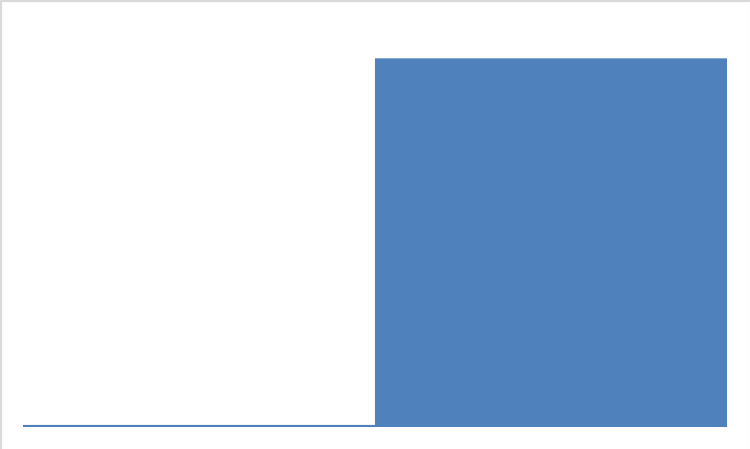
\includegraphics[width=0.2\textwidth, height=10mm]{methodology/images/mut17q21}\\
\textbf{loss 17} & 3 &  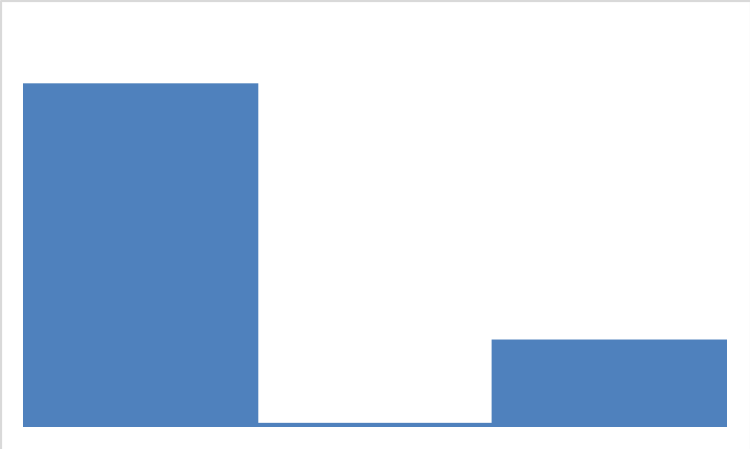
\includegraphics[width=0.2\textwidth, height=10mm]{methodology/images/loss_17}\\
\textbf{eta arrotondata} & 74 &  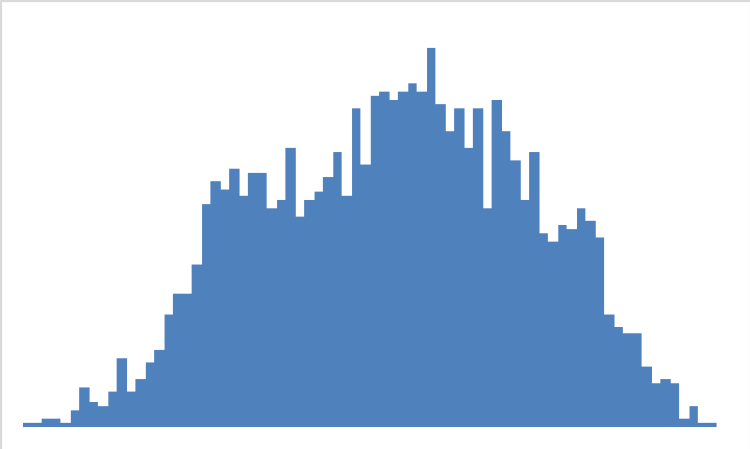
\includegraphics[width=0.2\textwidth, height=10mm]{methodology/images/eta_arrotondata}\\
\textbf{lateralit\`a} & 3 & 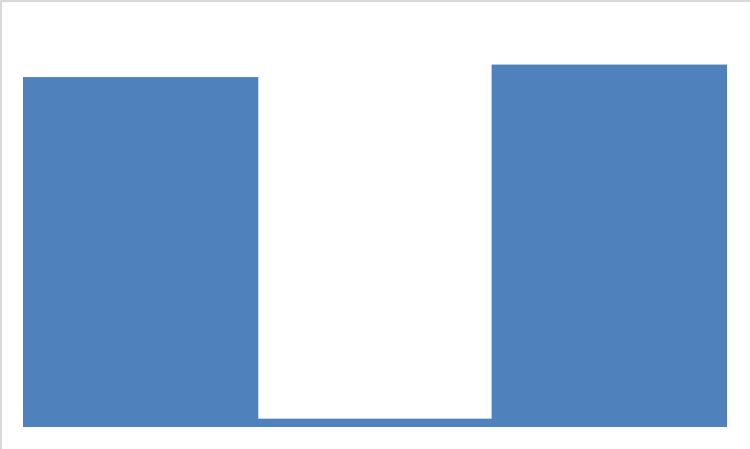
\includegraphics[width=0.2\textwidth, height=10mm]{methodology/images/lateralita} \\
\textbf{situ} & 5 & 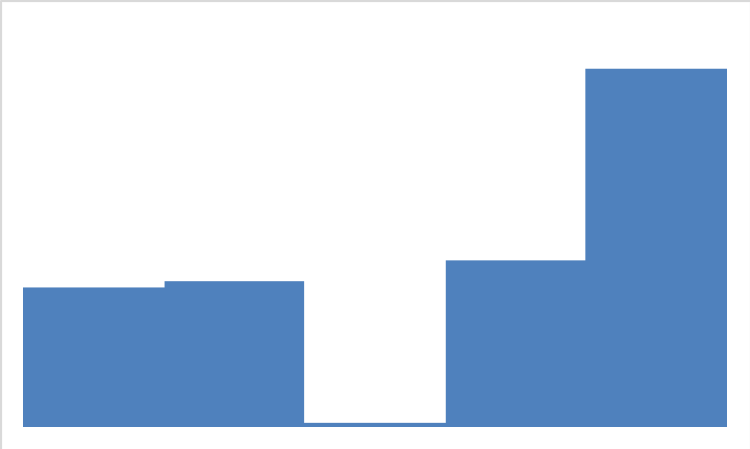
\includegraphics[width=0.2\textwidth, height=10mm]{methodology/images/situ} \\
\textbf{morfologia} & 5 & 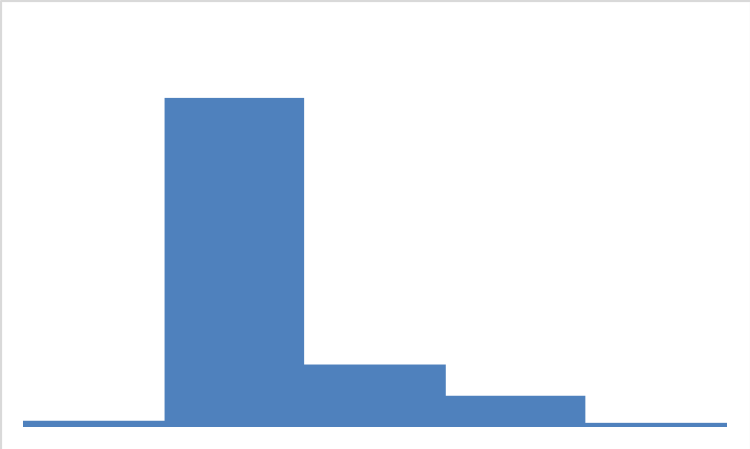
\includegraphics[width=0.2\textwidth, height=10mm]{methodology/images/morfologia} \\
\textbf{pT} & 23 & 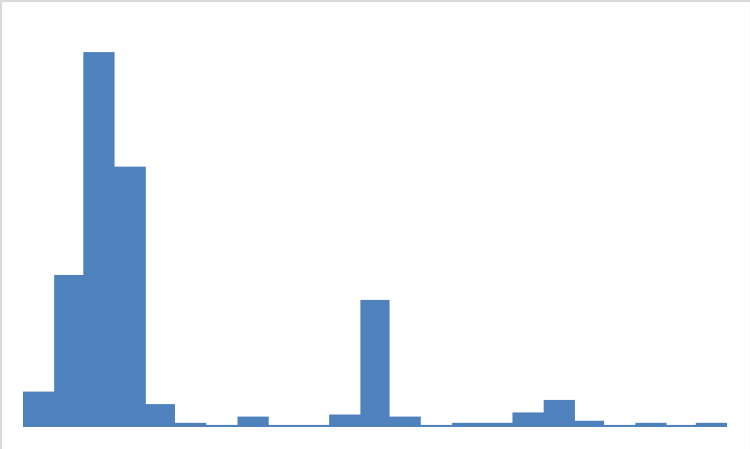
\includegraphics[width=0.2\textwidth, height=10mm]{methodology/images/pt} \\
\textbf{pN} & 6 & 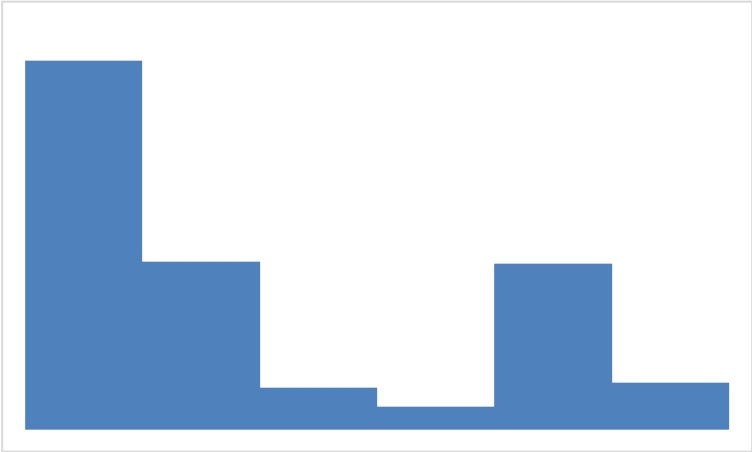
\includegraphics[width=0.2\textwidth, height=10mm]{methodology/images/pn} \\
\textbf{M} & 3 & 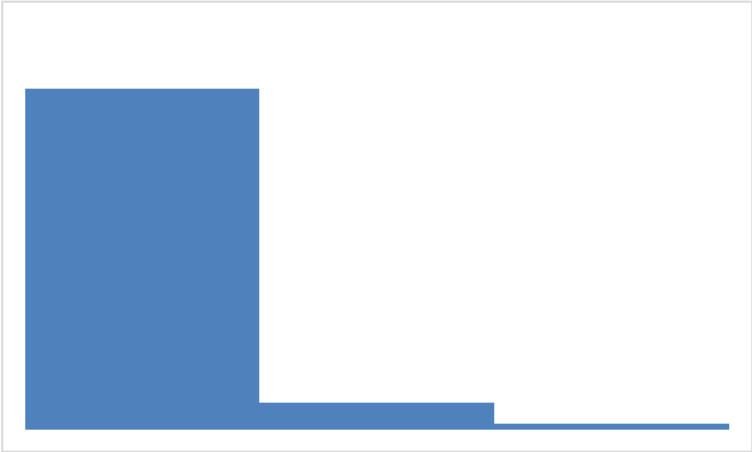
\includegraphics[width=0.2\textwidth, height=10mm]{methodology/images/m} \\
\textbf{differenziazione} & 5 & 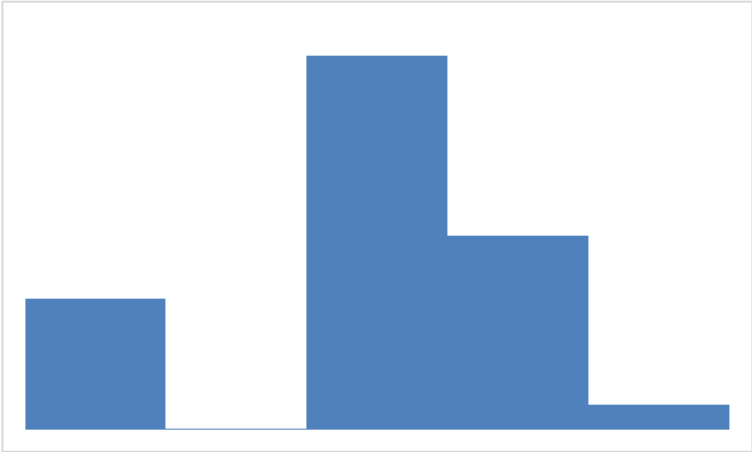
\includegraphics[width=0.2\textwidth, height=10mm]{methodology/images/differenziazione}  \\
\textbf{recettori estrogeni} & 40 & 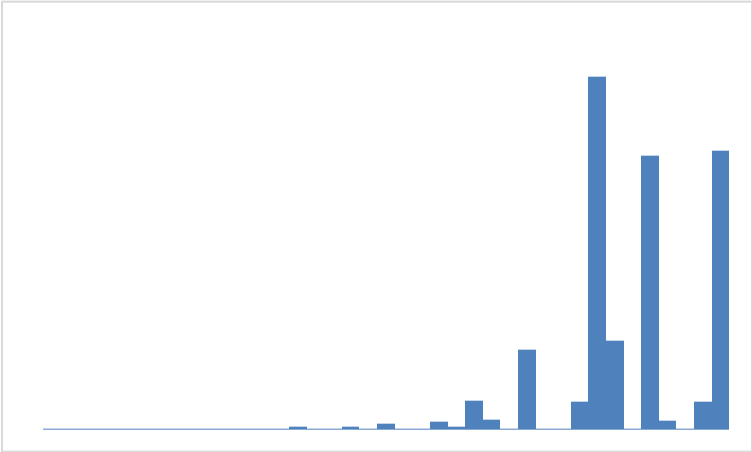
\includegraphics[width=0.2\textwidth, height=10mm]{methodology/images/recettori_estrogeni} \\
\textbf{recettori progestinici} & 40 & 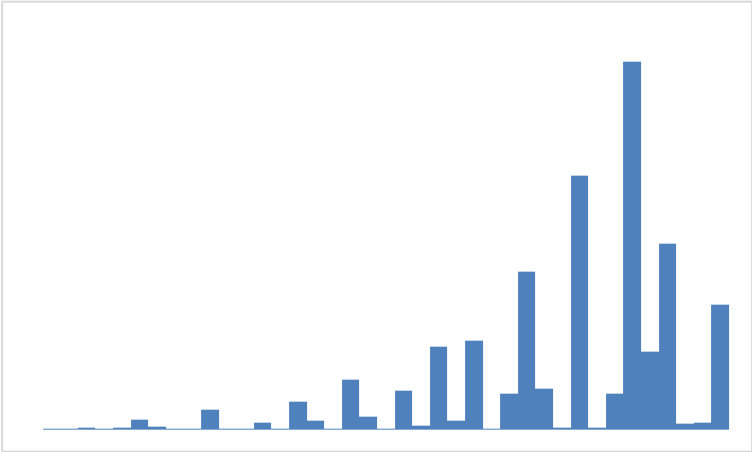
\includegraphics[width=0.2\textwidth, height=10mm]{methodology/images/recettori_progestinici}\\
\textbf{c erbB 2} & 4 & 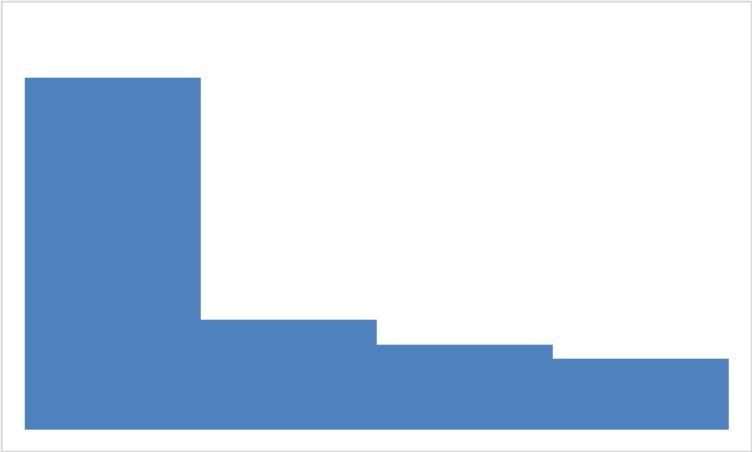
\includegraphics[width=0.2\textwidth, height=10mm]{methodology/images/c_erb_2}\\
\textbf{Ki67} & 52 & 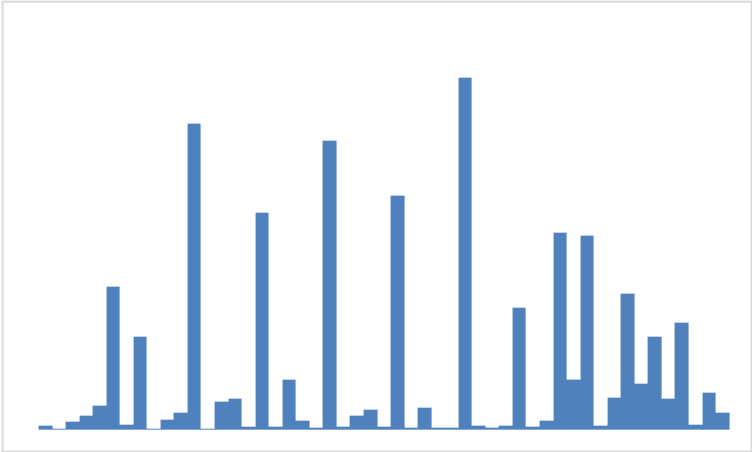
\includegraphics[width=0.2\textwidth, height=10mm]{methodology/images/ki67}\\
\textbf{FISHRation} & 5 &  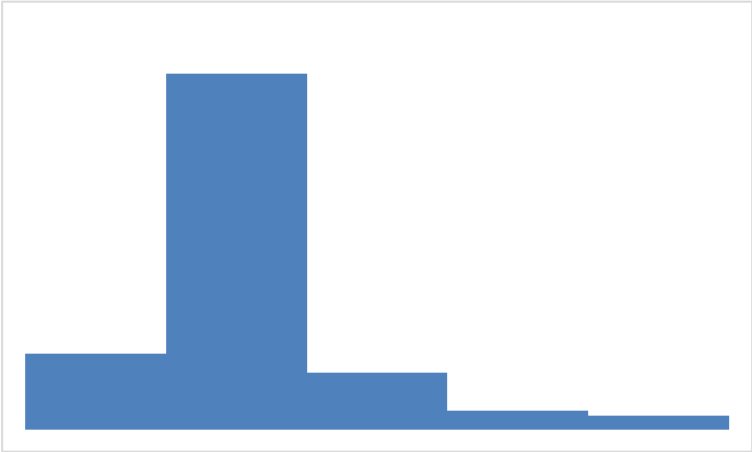
\includegraphics[width=0.2\textwidth, height=10mm]{methodology/images/fish}\\
\bottomrule
\end{tabularx}
\label{tab:datasetdistribution}
\end{table*}

\begin{table*}[htbp]
\centering
\caption{Data set preprocessing steps}
\begin{tabularx}{\textwidth}{@{} l Y @{}}
\toprule 
\textbf{Variable} & Action \\
\midrule 
\textbf{Codice globale} & Remove variable \\
\textbf{mut17q21} & Remove variable \\
\textbf{loss 17} & Remove variable \\
\textbf{eta arrotondata} & Bin into \enquote{$< 40$}, \enquote{$40-50$}, \enquote{$\geq 50$} \\
\textbf{lateralita} & Remove blanks and \enquote{sconosciuta} \\
\textbf{situ} & Remove blanks \\ \addlinespace
\textbf{morfologia} & Remove blanks and \enquote{unuseful} if performance on classification is subpar \\ \addlinespace
\textbf{pT} & Remove blanks and \enquote{unuseful}  \\
\textbf{pN} & Remove blanks and bin into \enquote{0} and \enquote{$\neq0$}\\
\textbf{M} & Remove blanks \\ 
\textbf{differenziazione} & Remove blanks and \enquote{Sconosciuto o non applicabile} \\ \addlinespace
\textbf{recettori estrogeni} & Remove blanks and bin into \enquote{negativo} if $\leq 10$,
		\enquote{debolmente positivo} if $\leq 50$, 
		\enquote{fortemente positivo} if $> 50$ \\ \addlinespace
\textbf{recettori progestinici} & Remove blanks and bin into \enquote{negativo} if $\leq 10$, 
		\enquote{debolmente positivo} if $\leq 50$, 
		\enquote{fortemente positivo} if $> 50$ \\ \addlinespace
\textbf{c erbB 2} & Remove blanks \\ 
\textbf{ki67} & Remove blanks and bin into \enquote{<14}, 
		\enquote{14-20}, \enquote{20-30}, \enquote{>30} \\ 
\textbf{FISH} & Remove variable \\
\bottomrule
\end{tabularx}
\label{tab:datasetpreprocess}
\end{table*}

